%%%%%%%%%%%%%%%%%%%%%%%%%%%%%%%%%%%%%%%%%
% Short Sectioned Assignment
% LaTeX Template
% Version 1.0 (5/5/12)
%
% This template has been downloaded from:
% http://www.LaTeXTemplates.com
%
% Original author:
% Frits Wenneker (http://www.howtotex.com)
%
% License:
% CC BY-NC-SA 3.0 (http://creativecommons.org/licenses/by-nc-sa/3.0/)
%
%%%%%%%%%%%%%%%%%%%%%%%%%%%%%%%%%%%%%%%%%

%----------------------------------------------------------------------------------------
%	PACKAGES AND OTHER DOCUMENT CONFIGURATIONS
%----------------------------------------------------------------------------------------

\documentclass[paper=a4, fontsize=11pt]{scrartcl} % A4 paper and 11pt font size

\usepackage[T1]{fontenc} % Use 8-bit encoding that has 256 glyphs
%\usepackage{fourier} % Use the Adobe Utopia font for the document - comment this line to return to the LaTeX default
\usepackage[english]{babel} % English language/hyphenation
\usepackage{amsmath,amsfonts,amsthm} % Math packages
\usepackage{hyperref} %HTML package
\usepackage{pgfplots} %Makes plots in LaTeX
\usepackage{tikz} %Also tikz?
\usepgfplotslibrary{fillbetween}%Let's me fill between named plots


\usepackage{sectsty} % Allows customizing section commands
\allsectionsfont{ \normalfont\scshape} % Make all sections the default font and small caps


\renewcommand{\thesubsection}{\alph{subsection}} %Make subsections start with letters

\usepackage{fancyhdr} % Custom headers and footers
\pagestyle{fancyplain} % Makes all pages in the document conform to the custom headers and footers
\fancyhead{} % No page header - if you want one, create it in the same way as the footers below
\fancyfoot[L]{} % Empty left footer
\fancyfoot[C]{} % Empty center footer
\fancyfoot[R]{\thepage} % Page numbering for right footer
\renewcommand{\headrulewidth}{0pt} % Remove header underlines
\renewcommand{\footrulewidth}{0pt} % Remove footer underlines
\setlength{\headheight}{13.6pt} % Customize the height of the header

\numberwithin{equation}{section} % Number equations within sections (i.e. 1.1, 1.2, 2.1, 2.2 instead of 1, 2, 3, 4)
\numberwithin{figure}{section} % Number figures within sections (i.e. 1.1, 1.2, 2.1, 2.2 instead of 1, 2, 3, 4)
\numberwithin{table}{section} % Number tables within sections (i.e. 1.1, 1.2, 2.1, 2.2 instead of 1, 2, 3, 4)

\setlength\parindent{0pt} % Removes all indentation from paragraphs - comment this line for an assignment with lots of text

%----------------------------------------------------------------------------------------
%	TITLE SECTION
%----------------------------------------------------------------------------------------

\newcommand{\horrule}[1]{\rule{\linewidth}{#1}} % Create horizontal rule command with 1 argument of height

\title{	Assignment 2}

\author{Benjamin Jakubowski} % Your name

\date{\normalsize\today} % Today's date or a custom date

\begin{document}

\maketitle % Print the title

%----------------------------------------------------------------------------------------
%	PROBLEM 1
%----------------------------------------------------------------------------------------

\section{Spider on a Wall}

\subsection{Position of Spider on Wall}

Let $F_{X, Y}(x,y)$ be the pdf. Then, since the spider spends twice as much time under the painting than it does on the rest of the wall,
\begin{equation*}
\int_{y=6}^8\int_{x=4}^6{f_{X, Y}(x,y) \textrm{d}x \textrm{d}y} = 2/3
\end{equation*}

The spider is equally likely to be anywhere under the painting, so $f_{X, Y}(x,y) = c$ and
\begin{align*}
\int_{y=6}^8\int_{x=4}^6{f_{X, Y}(x,y) \textrm{d}x \textrm{d}y} &= 2/3 \\
\int_{y=6}^8\int_{x=4}^6{c \textrm{d}x \textrm{d}y} &= 2/3 \\
\int_{y=6}^8{2c \textrm{d}y} &= 2/3 \\
4c &= 2/3
\end{align*}

Thus $c = 1/6$. Now let $S$ be the region of the wall not under the painting. Note $Area_{S} = 96$, and 
\begin{equation*}
\int_{\{(x,y) \in S\}}f_{X, Y}(x,y) \textrm{d}x \textrm{d}y =1/3
\end{equation*}

Since the spider is equally likely to be anywhere in $S$, 
\begin{align*}
\int_{\{(x,y) \in S\}}f_{X, Y}(x,y) \textrm{d}x \textrm{d}y &=1/3 \\
\int_{\{(x,y) \in S\}}k \textrm{d}x \textrm{d} y &=1/3 \\
k \int_{\{(x,y) \in S\}}1 \textrm{d}x \textrm{d} y &=1/3 \\
k * Area_{S} &= 1/3 \\
k * 96 &= 1/3
\end{align*}

So $k = 1/288$. Thus, (with $S$ defined as above), 
\[ 
f_{X,Y}(x,y) = 
	\begin{cases}
		1/6 & \textrm{if } 4 \leq x \leq 6, 6 \leq y \leq 8 \\
		1/288 & \textrm{if } (x,y) \in S\\
		0 & \textrm{otherwise}
	\end{cases}
\]

\subsection{Height of spider on wall}
The pdf of the height is just the marginal pdf $f_{Y}(y)$,
\begin{align*}
f_{Y}(y) &= \int_{x=-\infty}^\infty f_{X, Y}(x,y) \textrm{d}x \\
   &= \int_0^{10} f_{X, Y} (x,y) \textrm{d}x
\end{align*}

since $f_{X, Y}(x,y) = 0$ for $0<x, 10<x$.

Then, for $0 \leq y < 6$,

\begin{equation*}
f_Y(y) = \int_0^{10} f_{X, Y}(x,y) \textrm{d}x =  \int_0^{10} 1/288 \textrm{d}x = 10/288
\end{equation*}

For $6 \leq y \leq 8$,

\begin{align*}
f_Y(y) &= \int_0^{10} f_{X, Y}(x,y) \textrm{d}x\\
   &= \int_0^4 f_{X, Y}(x,y) \textrm{d}x + \int_4^6 f_{X, Y}(x,y) \textrm{d}x +\int_6^{10} f_{X, Y}(x,y) \textrm{d}x  \\
      &= \int_0^4 1/288 \textrm{d}x + \int_4^6 1/6 \textrm{d}x +\int_6^{10} 1/288 \textrm{d}x  \\
      &= 4/288 + 2/6 + 4/288 = 104/288
\end{align*}

For $8 < y \leq 10$,

\begin{equation*}
f_Y(y) = \int_0^{10} f_{X, Y}(x,y) \textrm{d}x =  \int_0^{10} 1/288 \textrm{d}x = 10/288
\end{equation*}

Thus,
\[ 
f_Y(y) = 
	\begin{cases}
		10/288 & \textrm{if } 0 \leq y <6 \\
		104/288 & \textrm{if } 6 \leq y \leq 8\\
		10/288 & \textrm{if } 8 < y \leq 10
	\end{cases}
\]

This pdf is plotted below\footnote{This plot was generated using code adapted from \href{http://gma.math.ufl.edu/files/tikz.pdf}{"Graphing in \LaTeX using PGF and TikZ"} by Lauderdale and Gluck}:

\begin{center}
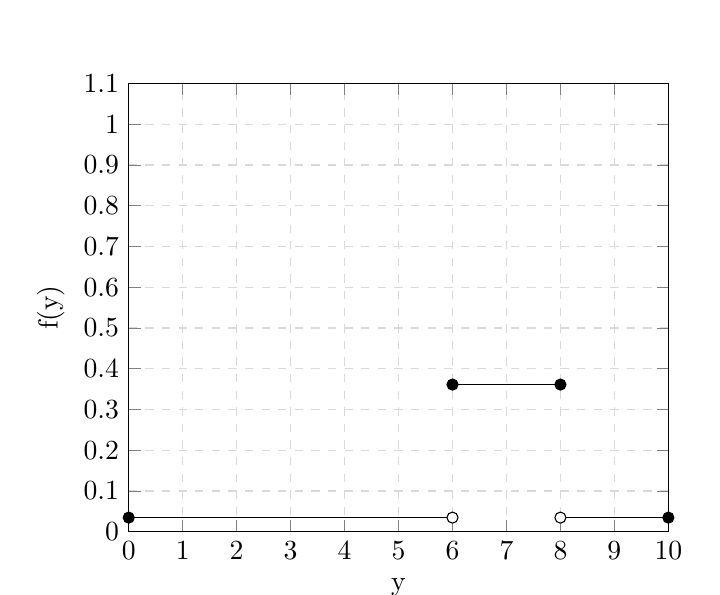
\begin{tikzpicture}
	\begin{axis}[xtick={0,...,10}, ytick={0,0.1,0.2,0.3,0.4,0.5,0.6,0.7,0.8,0.9,1,1.1}, xmin=0, xmax=10, ymin=0, ymax=1.1, xlabel=y, ylabel={f(y)}, grid=major, grid style={dashed,gray!30}]
	  \addplot[domain=0:6] {10/288};
          \addplot[domain=6:8] {104/288};
          \addplot[domain=8:10] {10/288};
	  
	  \addplot[mark=*] coordinates {(0,10/288)};
	  \addplot[mark=*,fill=white] coordinates {(6,10/288)};
	  \addplot[mark=*] coordinates {(6,104/288)};
	  \addplot[mark=*] coordinates {(8,104/288)};
	  \addplot[mark=*,fill=white] coordinates {(8,10/288)};
	  \addplot[mark=*] coordinates {(10,10/288)};
	\end{axis}
\end{tikzpicture}
\end{center}

\subsection{CDF of height, given spider is visible}

Recall the set $S$ is the visible area of the wall, and that $P((x,y)\in S) = 1/3$. The conditional cdf of the height $Y$, given we see the spider (i.e. $Y \in S$), is given by:

\begin{equation*}
f_{Y | {Y \in S}} (u) = \frac{\int_{y=0}^u \int_{\{x | (x,y) \in S \}} f_{X,Y}(x,y)\textrm{d}x\textrm{d}y}{P((x,y)\in S)} = \frac{\int_{y=0}^u \int_{\{x | (x,y) \in S \}} f_{X,Y}(x,y)\textrm{d}x\textrm{d}y}{1/3}
\end{equation*}

Thus
\[ 
f_{Y | {Y \in S}} (u) = 
	\begin{cases}
		\frac{\int_0^u f_Y(y) \textrm{d}y}{1/3} & \textrm{if } 0 \leq u <6 \\
		\\
		\frac{\int_0^6 f_Y(y) \textrm{d}y +\int_6^u \int_0^4 f_{X, Y}(x,y) \textrm{d}x\textrm{d}y + \int_6^u \int_6^{10} f_{X, Y}(x,y) \textrm{d}x\textrm{d}y }{1/3} & \textrm{if } 6 \leq u \leq 8\\
		\\
		\frac{\int_0^6 f_Y(y) \textrm{d}y +\int_6^8 \int_0^4 f_{X, Y}(x,y) \textrm{d}x\textrm{d}y + \int_6^8 \int_6^{10} f_{X, Y}(x,y) \textrm{d}x\textrm{d}y +\int_8^u f_Y(y) \textrm{d}y}{1/3} & \textrm{if } 8 < u \leq 10
	\end{cases}
\]

Evaluating these integrals yields
\[ 
f_{Y | {Y \in S}} (u) = 
	\begin{cases}
		\frac{10/288 u}{96/288} = 10/96 u & \textrm{if } 0 \leq u <6 \\
		\\
		\frac{60/288 + 4/288(u-6) + 4/288(u-6)}{1/3} = 
		\frac{8/288 u +12/288}{96/288} = 8/96 u + 12/ 96 & \textrm{if } 6 \leq u \leq 8\\
		\\
		\frac{76/288 + 10/288(u-8)}{96/288}  = 10/96 u - 4/96 & \textrm{if } 8 < u \leq 10
	\end{cases}
\]

This conditional cdf is plotted below:

\begin{center}
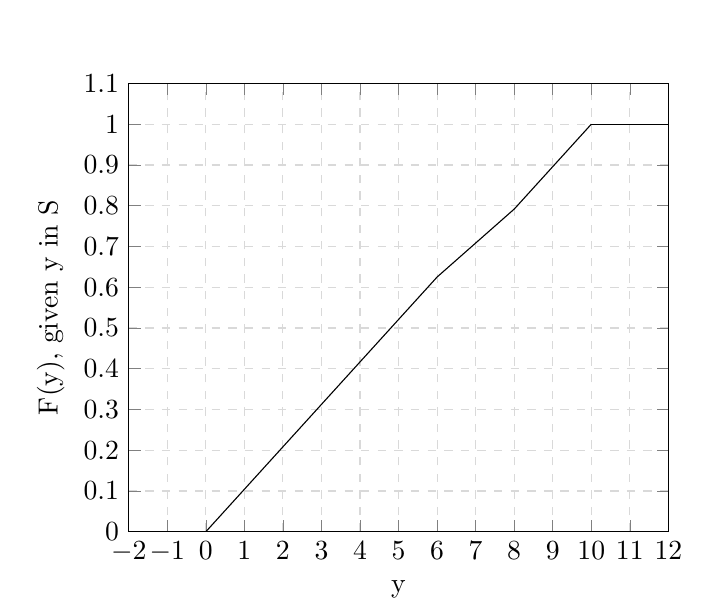
\begin{tikzpicture}
	\begin{axis}[xtick={-2,...,12}, ytick={0,0.1,0.2,0.3,0.4,0.5,0.6,0.7,0.8,0.9,1,1.1}, xmin=-2, xmax=12, ymin=0, ymax=1.1, xlabel=y, ylabel={F(y), given y in S}, grid=major, grid style={dashed,gray!30}]
	 \addplot[domain=-2:0] {0};
	 \addplot[domain=0:6] {10/96*x};
          \addplot[domain=6:8] {8/96*x + 12/96};
          \addplot[domain=8:10] {10/96*x - 4/96};
	  \addplot[domain=10:12] {1};
	\end{axis}
\end{tikzpicture} 
\end{center}

%----------------------------------------------------------------------------------------
%	PROBLEM 2
%----------------------------------------------------------------------------------------

\section{Pizza Delivery}

\subsection{Wait time- Pat or Robbie get called}

Let $X_P, X_R \sim Exp(\lambda)$ model the wait time until Pat and Robbie get calls, respectively. Then the wait time until one of them gets a call is $Z = \textrm{min}\{X_P, X_R\}$. Then,
\begin{align*}
F_Z(z) &= P(Z \leq z) = 1 - P(z < Z) \\
   &= 1 - P(z < X_P, z < X_R)
\end{align*}
Now, let's assume $X_R$ and $X_P$ are independent. This is a reasonable assumption if the market is large. At the lower limit for market size, imagine there is only a single customer who wants one pizza. Then, if they call Pat, they don't call Robbie (and vice versa), so obviously $X_R$ and $X_P$ are not independent. On the other hand, if the market is large and customers act independently of each other, $X_R$ and $X_P$ can reasonably be assumed to be independent. Then
\begin{align*}
F_Z &= 1 - P(z < X_P, z < X_R) \\
   &= 1- P(z < X_P)P(z < X_R)\\
   &= 1 - (1 - F_{X_P}(z))(1 - F_{X_R}(z))\\
   &= 1 - (1 - F_{X_P}(z)- F_{X_R}(z) + F_{X_P}(z)F_{X_R}(z))\\
   &= F_{X_P}(z) + F_{X_R}(z) - F_{X_P}(z)F_{X_R}(z)\\
   &= (1 - e^{-\lambda z}) + (1 - e^{-\lambda z}) - (1 - e^{-\lambda z})(1 - e^{-\lambda z})\\
   &= 1 - e^{-2\lambda z}
\end{align*}
Thus, $Z \sim Exp(2\lambda)$. This makes intuitive sense- if you expect calls to come into each store at a rate of $\lambda$, then you expect the combined rate of calls into both stores to be $2 \lambda$.

\subsection{Wait time- Pat and Robbie get called}

The distribution of the time until both Pat and Robbie have received a call is modeled by $W = \textrm{max}\{X_R, X_P\}$. Thus,
\begin{align*}
F_W(W) &= P(W \leq w)\\
   &= P(X_P \leq w, X_R \leq w)\\
   &= P(X_P \leq w)P(X_R \leq w) \textrm{   (again assuming independence)}\\
   &= F_{X_P}(w)F_{X_R}(w)\\
   &= 1 - 2 e^{-\lambda w} + e^{-2 \lambda w}
\end{align*}
\subsection{Comparing distributions}

Color-coded plots of the CDFs (with $\lambda = 1$) are given below, with \textcolor{red}{red} for \textcolor{red}{$F_X(t)$},  \textcolor{blue}{blue} for \textcolor{blue}{$F_Z(t)$}, and  \textcolor{green}{green} for \textcolor{green}{$F_W(t)$}.

\begin{center}
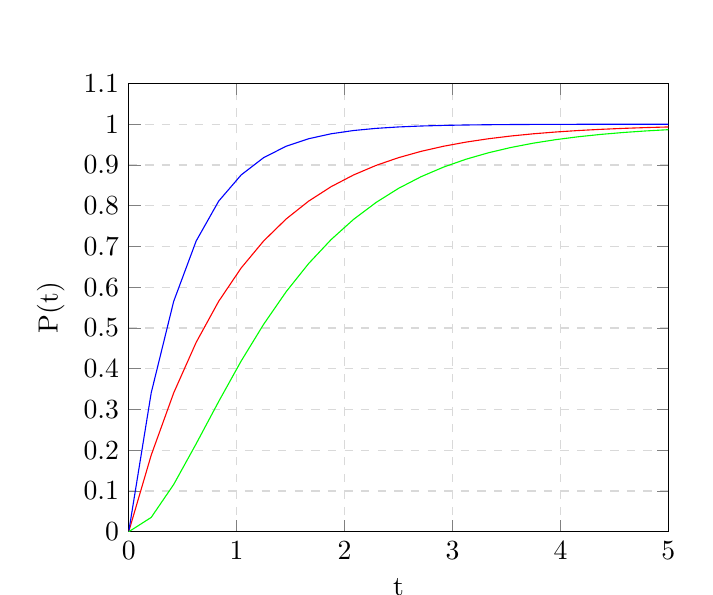
\begin{tikzpicture}
	\begin{axis}[xtick={0,...,5}, ytick={0,0.1,0.2,0.3,0.4,0.5,0.6,0.7,0.8,0.9,1,1.1}, xmin=0, xmax=5, ymin=0, ymax=1.1, xlabel=t, ylabel={P(t)}, grid=major, grid style={dashed,gray!30}]
	  \addplot[color=red,domain=0:5] {1-exp(-1*x)};
          \addplot[color=blue,domain=0:5] {1-exp(-2*x)};
          \addplot[color=green,domain=0:5] {1-2*exp(-1*x)+exp(-2*x)};
	\end{axis}
\end{tikzpicture}
\end{center}

These results make sense, when you observe the functions are ordered over all $0 < t$. Specifically, $F_Z(t) > F_X(t) > F_W(t)$. That's expected since, during any time interval $(0,t)$, the event \{Pat gets a call $\cup$ Robbie gets a call\} $\supseteq$ \{Pat gets a call\} $\supseteq$ \{Pat gets a call $\cap$ Robbie gets a call\} (note this is obviously also true if we swap the names "Pat" and "Robbie").

%----------------------------------------------------------------------------------------
%	PROBLEM 3
%----------------------------------------------------------------------------------------

\section{Cars}

\subsection{Proof of Equation (1)}

To start, recall $P(\Omega) = 1$. Now let $X \sim B(n, 0.5)$. Then,

\begin{align*}
\sum_{k = 0}^n {{n}\choose{k}}(1/2)^k(1/2)^{n-k} &= 1\\
\sum_{k = 0}^n {{n}\choose{k}}(1/2)^n &= 1\\
(1/2)^n\sum_{k = 0}^n {{n}\choose{k}} &= 1\\
\sum_{k = 0}^n {{n}\choose{k}} &= 2^n
\end{align*}

\subsection{PMF of the combined total number of mechanical problems}

Let $X_1, X_2$ be IID poisson RVs, with parameter $\lambda$, modeling the number of mechanical failures in your car and your sister's car, respectively. 

Then $Y = X_1 + X_2$ is the total number of mechanical failures. Then
\begin{align*}
P(Y = y) &= P(X_1 + X_2 = y)\\
   &= \sum_{x_2 = 0}^y P(X_1 = y - x_2 | X_2 = x_2) P(X_2 = x_2)\\
   &=  \sum_{x_2 = 0}^y P(X_1 = y - x_2) P(X_2 = x_2) \textrm{      (by independence)}\\
   &= \sum_{x_2 = 0}^y \frac{\lambda^{y-x_2}}{(y-x_2)!}e^{-\lambda}\frac{\lambda^{x_2}}{(x_2)!}e^{-\lambda}\\
   &=  \sum_{x_2 = 0}^y \frac{y!}{x_2!(y-x_2)!}\lambda^y e^{-2\lambda}\frac{1}{y!}\\
   &=  \lambda^y e^{-2\lambda}\frac{1}{y!}\sum_{x_2 = 0}^y \frac{y!}{x_2!(y-x_2)!} =  \lambda^y e^{-2\lambda}\frac{1}{y!}\sum_{x_2 = 0}^y {{y}\choose{x_2}}\\
   &=  \lambda^y e^{-2\lambda}\frac{1}{y!} 2^y\\
   &=  \frac{(2\lambda)^y}{y!} e^{-2\lambda}\\
\end{align*}
Thus, $Y \sim Pois(2\lambda)$. Again, this makes intuitive sense- the Poisson distribution models the number of events occurring in a time interval, given a known rate $\lambda$. If we're adding two IID Poisson RVs, we'd expect this rate to double, but the underlying generating process to be otherwise unchanged.

%----------------------------------------------------------------------------------------
%	PROBLEM 4
%----------------------------------------------------------------------------------------

\section{Race}

\subsection{Joint PDF of the positions of Mary and Hannah}

First, let $M \sim U(0,10)$ and $H \sim U(0,10)$ represent the locations of Mary and Hannah respectively. Since M and H are IID, $f_{M, H}(m,h) = f_M(m)f_H(h)$. Thus

\[
f_{M,H}(m,h) = 
\begin{cases}
		\frac{1}{10-0}\frac{1}{10-0}=\frac{1}{100} & \textrm{if } 0 \leq H \leq 10, 0 \leq M \leq 10 \\
		0 & \textrm{otherwise}\\
\end{cases}
\]


This joint PDF is shown below (in section B). The boxed area represents $F_{M, H}(m,h)$ while the blue area represents the area in which $D \leq d=3$ (defined and discussed below).

\subsection{Shading area corresponding to $P(D \leq d)$}

First, let $D$ represent the distance between Mary and Hannah. To illustrate the area corresponding to $D \leq d$, let's let $d=3$. The corresponding area is shaded blue in the plot below.

\begin{center}
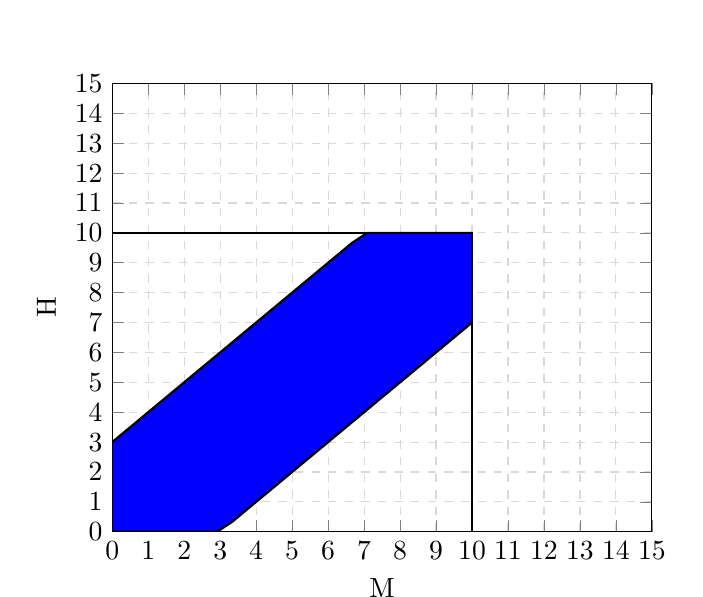
\begin{tikzpicture}
	\begin{axis}[xtick={0,...,15}, ytick={0,...,15}, xmin=0, xmax=15, ymin=0, ymax=15, xlabel=M, ylabel=H, grid=major, grid style={dashed,gray!30}]
        \draw[draw=black, thick] (axis cs:0,0) rectangle (axis cs:10,10);
	\addplot[name path=upper, thick, domain=0:10]{min(x+3,10)};
	\addplot[name path=lower, thick, domain=0:10]{max(x-3,0)};
	 \addplot [fill=blue] fill between[of = upper and lower];
	\end{axis}
\end{tikzpicture}
\end{center}

\subsection{Finding the PDF $F_D(d)$}

First, notice the area in $[0,10] \times [0,10]$ not covered by $D \leq d$ is $(10-d)^2$. Thus,
\begin{equation*}
F_D(d) = P(D \leq d) = 1 - P(D > d) = 1 - 1/100 * (10-d)^2
\end{equation*}
Thus
\begin{equation*}
f_D(d) = F_D'(d) = 1/5 - 1/50 d
\end{equation*}   
This CDF is plotted below:

\begin{center}
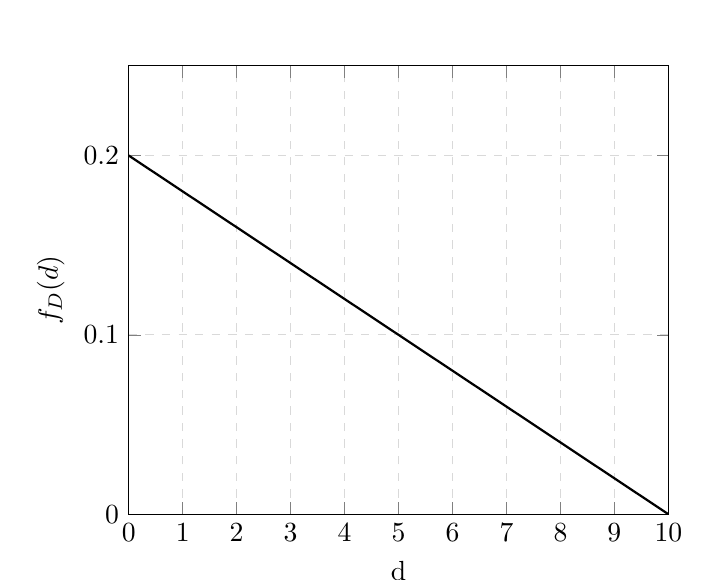
\begin{tikzpicture}
	\begin{axis}[xtick={0,...,10}, ytick={0,0.1,.2}, xmin=0, xmax=10, ymin=0, ymax=0.25, xlabel=d, ylabel=$f_D(d)$, grid=major, grid style={dashed,gray!30}]
      	\addplot[thick, domain=0:10]{1/5 - 1/50*x};
	\end{axis}
\end{tikzpicture}
\end{center}

Again, as a side note, observe this PDF makes intuitive sense- given $M$ and $H$ are IID uniform, it makes sense $f_D(d)$ has a maximum at $d=0$.

%----------------------------------------------------------------------------------------
%	PROBLEM 5
%----------------------------------------------------------------------------------------
\section{Cheating at coin flips}

\subsection{Probability of heads/tails}

First, let $X \sim \textrm{Bernouilli}(P)$ model the outcome of the coin flip. Let
\[
X = 
\begin{cases}
		1 & \textrm{if heads} \\
		0 & \textrm{if tails}\\
\end{cases}
\]
Then
\[
P_X(x) = 
\begin{cases}
		(1-P) & \textrm{for x =0} \\
		P & \textrm{for x= 1}\\
\end{cases}
\]
Since we suspect but do not know that the coin is biased, P is itself a $U(0.5,1)$ random variable. This is reasonable- if the coin is biased, we can assume it is biased in Marvin's favor (so $0.5 \leq P$), and (obviously)  $P \leq 1$. The probability the coin flip is heads under this model is:
\begin{align*}
P(X = 1) &= \int_{0.5}^1 P(X = 1 | P = p) f_P(p) \textrm{d}p\\
   &= \int_{0.5}^1 p \cdot f_P(p) \textrm{d}p \\
   &= \int_{0.5}^1 2p  \textrm{d}p = p^2\Big|_{p = 0.5}^1 = 1 - 0.25 = 0.75
\end{align*}

Thus, under this model, the probability of heads is 0.75 and the probability of tails is 0.25. As a side note, this again makes intuitive sense- $X$ is essentially an indicator variable, so $P(X = 1)$ is just the expected value $\textrm{E}[P] = 0.75$. 

\subsection{Updating our model}

We will use Bayes rule to update our model. If the coin flip is heads ($X = 1$), then
\begin{equation*}
f_{P | X}(p | 1) = \frac{P(X = 1 | P = p) \cdot f_P(p)}{\int_{0.5}^1P(X = 1 | P =  p) \cdot f_P(p) \textrm{d}p}
\end{equation*}
Recall $f_P(p) = 2 \textrm{ for } 0.5 \leq p \leq 1, \int_{0.5}^1P(X = 1 | P = p)\cdot f_P(p) \textrm{d}p = 0.75, \textrm{ and } \\ P(X=1 | P = p) = p$.
Thus, substitution yields
\begin{equation*}
f_{P | X}(p | 1) = \frac{p \cdot 2}{0.75} = 8/3 p
\end{equation*}

Next, if the coin flip is tails, ($X = 0$), then
\begin{align*}
f_{P | X}(p | 0) &= \frac{P(X = 0 | P = p) \cdot f_P(p)}{\int_{0.5}^1P(X = 0 | P =  p) \cdot f_P(p) \textrm{d}p}\\
   &= \frac{(1-p)\cdot 2}{0.25}\\
   &= 8(1-p)
\end{align*}

Thus, the conditional PDF $f_{P | X}(p | x)$ is
\[
f_{P | X}(p | x) = 
\begin{cases}
		8/3 p & \textrm{for x = 1 (flip 1 is heads)} \\
		8 (1-p) & \textrm{for x = 0 (flip 1 is tails)}\\
\end{cases}
\]

Below are color-coded plots of these posterior PDFs, and the prior PDF $f_P(p)$, with \textcolor{red}{red} for \textcolor{red}{$f_P(p)$},  \textcolor{blue}{blue} for \textcolor{blue}{$f_{P | X} (p | 1)$}, and  \textcolor{green}{green} for \textcolor{green}{$f_{P | X} (p | 0)$}.

\begin{center}
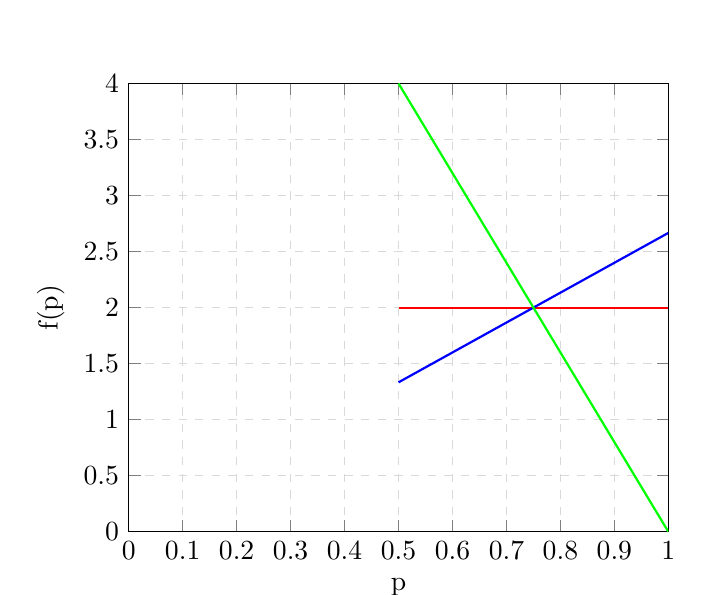
\begin{tikzpicture}
	\begin{axis}[xtick={0,0.1,0.2,0.3,0.4,0.5,0.6,0.7,0.8,0.9,1}, ytick={0,0.5,...,4}, xmin=0, xmax=1, ymin=0, ymax=4, xlabel=p, ylabel={f(p)}, grid=major, grid style={dashed,gray!30}]
	  \addplot[thick, color=red,domain=0.5:1] {2};
          \addplot[thick, color=blue,domain=0.5:1] {8/3*x};
          \addplot[thick, color=green,domain=0.5:1] {8*(1-x))};
	\end{axis}
\end{tikzpicture}
\end{center}

These posterior PDFs make sense. If our first flip returns a head, then we become more confident  the coin is in fact biased. On the other hand, if our first flip returns a tail, then we are less confident the coin is biased. To see this more clearly, we can consider the expected value of the two posterior distributions:
\begin{align*}
\textrm{E}[P | X = 0] = \int_{0.5}^1 p \cdot 8(1-p) \textrm{d}p = 2/3 = 0.\bar{6}\\
\textrm{E}[P | X = 1] = \int_{0.5}^1 p \cdot 8/3 p \textrm{d}p = 7/9 = 0.\bar{7}
\end{align*}
Recall the our prior expectation $\textrm{E}[P] = 0.75$. Thus, if the first flip is a tails, we revise our expected value for the bias downwards considerably. On the other hand, if the first flip is a heads, we revise our expected value for the bias up only slightly. This is also visible in the plots of the PDFs- the change in the slope of the PDF if tails is much greater than the change in the slope if heads.

%----------------------------------------------------------------------------------------


\end{document}